
\begin{abstract}

A diabetes diagnosis entails important consequences for its recipients. They obtain health information but also face the challenge of having to manage the condition via lifestyle adjustments, with potential consequences for---among other things---their economic activity. We investigate the causal effect of a diabetes diagnosis on behavioural risk-factors as well as on employment chances, two potentially intertwined factors. We used longitudinal data from the \acf{CHNS}, covering the years 1997 to 2011. Two complementary statistical techniques---marginal structural models and fixed effects panel estimation---were used to estimate the causal effect of a diabetes diagnosis on a series of behavioural risk-factors and employment probabilities. Both models suggest female employment chances to decline significantly as a result of a diabetes diagnosis (over 11 percentage points), but no adverse effects for men. Chinese men appear to respond to a diagnosis by significantly reducing their \ac{BMI}, waist circumference and calorie consumption, in ways that are sustained over time. The effects on behavioural outcomes for women are smaller and less consistent. In light of the results it may be worthwhile for the Chinese healthcare system to focus efforts on addressing the needs of women with diabetes as it is them who have particular difficulties in improving their behavioural risk factors and who---perhaps as a consequence---pay the biggest price in terms of loss of employment chances. Future research is needed to unravel the mechanism behind these sex differences.


\end{abstract}


\section{\label{sec:Introduction5}Introduction}

Diabetes risk factors such as alcohol consumption, weight gain, smoking or caloric consumption are all related to the onset of diabetes as well as ensuing diabetes complications. They may further be influenced by the diabetes diagnosis itself as well as by a person's employment status. Research shows for instance that behaviour changes after a diabetes diagnosis can have positive health effects and reduce the risk of subsequent cardiovascular events\parencite{Long2014}, may help in effectively managing blood glucose levels and achieving further treatment goals \parencite{Zhou2016}. As a consequence, such changes may also affect the economic impact of diabetes if they cause a delay in or even prevent the onset of complications. Further, employment status may itself be related to diabetes risk factors, for example by affecting the time spend on physical activity or by increasing stress levels due to unemployment or due to challenges at the workplace, affect other risk behaviours such as smoking or alcohol consumption. In an effort to longitudinally investigate the impact of unemployment on health behaviours, \textcite{Colman2014} found heterogeneous effects of unemployment, with it leading to slight weight gain, a decrease in smoking and decreases in fast-food consumption. Macroeconomic evidence also indicates that job loss can lead to changes in health, especially in mental health \parencite{Charles2008}, which may have further downstream effects on health behaviours.

Research on the impact of diabetes on labour market outcomes has so far ignored the potentially simultaneous relationship of diabetes, employment and behavioural diabetes risk factors due to the danger of over-adjusting, as standard regression techniques such as \ac{OLS} or \ac{FE} are unable to account for multi-directional relationships. Similarly, there is a dearth of studies investigating longitudinally the impact of a diabetes diagnosis on behavioural diabetes risk factors, while taking into account the effect of employment status on both diabetes and diabetes risk factors. A further challenge faced by researchers investigating the effects of diabetes on both economic outcomes and risk factors are unobserved variables that may be biasing the estimates. In particular time-invariant ones such as poor early life conditions or time stable personal character trades, may simultaneously increase the probabilities to develop diabetes and to be unemployed or to engage in unhealthy behaviours. 

The goal of this study is therefore to assess the impact of a diabetes diagnosis on both employment probabilities and behavioural risk factors while accounting for the potentially intertwined relationships between diabetes, employment and health behaviours. This is done via the use of \acp{MSM}, an estimation strategy that is able to account for time-dependent confounding across time \parencite{Robins2000} when estimating the impact of a treatment, here a diabetes diagnosis, on the outcome of interest. This is the first time this strategy is used to estimate the impact of diabetes on employment status. We further complement this and test the robustness of \ac{MSM} to the potential violation of one of its crucial assumptions of no unmeasured confounding. Therefore, we estimate \acp{FE} models that---while unable to account for the potentially simultaneous relationships---are able to take into account any unobserved time-invariant confounding additionally to confounding due to observed variables. Very different results to the \ac{MSM} would suggest considerable unobserved confounding. To assess further how important any unmeasured confounding may be, we additionally estimate \ac{RE} models to compare the results from the \acp{MSM} and \ac{FE} models against. Apart from these methodological contributions, the study also further extends the evidence base for the impact of diabetes on employment probabilities in \acp{MIC}, where currently empirical information is only available for Mexico \parencite{Seuring2016}. At the same time the study provides first, as far as we are aware, longitudinal evidence for the effect of a diabetes diagnosis on behavioural risk factors for diabetes complications in China or any \ac{LMIC} for that matter.

 
More information about the effects of a diabetes diagnosis may be particularly important for \acp{LMIC} such as China, where diabetes prevalence has surged from 1\% in the early 1980s to about 10\% in recent years \autocite{Hu2011,Risk2016}. Confronting this diabetes epidemic puts a strain on healthcare systems \parencite{Seuring2015a}, increasing the need to find highly cost-effective prevention and treatment options in very resource constraint settings \parencite{WHOresearchpriorities2010}. However, to do this it is important to assess how successful people with diabetes currently are in preventing adverse economic effects and reducing their risk factors for diabetes complications.

So far, population-level longitudinal research on the effects of health information on post-diagnosis behaviour change is scarce and has been limited to \acp{HIC}. The sole study on the effects of recently diagnosed diabetes on health behaviours found positive behaviour changes shortly after diagnosis in a USA population. However, the effects were mostly short lived and tended to dissipate over time, particularly considering weight loss \autocite{Slade2012}. Slade created an "at risk" control group without diabetes that intended to be similar to the treatment group with diabetes, apart from not having received a diagnosis. He used information on diabetes biomarkers to estimate the propensity score of those without a diabetes diagnosis to be above a specific at risk threshold, so that everybody above a certain propensity score was used to form the control group. He then estimated dynamic population averaged as well as \ac{FE} models for identification. While this allowed for the construction of a control group, the study was not able to account for the bidirectional relationship between diabetes and health behaviours.

Another study investigated the effect of a hypertension diagnosis on nutritional behaviours in China using a regression-discontinuity design and biomarker information on blood pressure \autocite{Zhao2013a}. A crucial assumption in the study was that people above the hypertension threshold were indeed informed about that outcome while those just below the threshold were not. These two groups were then compared to isolate the particular effect of the additional health information on food consumption. The results indicated that a diagnosis leads to reductions in fat consumption at the consecutive wave, though only for those economically better off. However, an important caveat of the study was that it was not always clear whether the participants received just the actual blood pressure measurement information and had to interpret these data themselves, or whether they were made explicitly aware of their hypertension (or also pre-hypertension) status \autocite{Zhao2013a}. Further, the results may have limited generalisability, since the measured treatment effect is a very local one, applying only to the population around the hypertension threshold. The effects may have been different for people receiving their 'diagnosis' while already having very severe hypertension.

%Finally, another study on China also used diabetes biomarkers to identify those formally unaware of their diabetes, assuming that they were informed about their diabetes status by the survey team \parencite{Liu2014}. They use a difference in difference approach to identify the effect of a diagnosis on labour income in the wave after diagnosis, finding a decrease of about 16\%. They attribute this effect to the psychological consequences of the diabetes diagnosis, however, they are not able to rule out an effect of a deterioration of health on income. Further, the results only provide a short term picture, and it remains unclear if people are able to recover from the initial shock. ONLY INCLUDE IF I ALSO LOOK AT INCOME

This study adds in several ways to the existing literature. First, it shows the impact of diabetes diagnosis on labour outcomes in China, not only over the short term, but for a period covering the entire decade of the 2000s, allowing for a more long term investigation of the effects. This both confirms and extends earlier evidence for other settings and using different methods. Second, it provides information on the effect of a diabetes diagnosis on health behaviours. Third, by considering the effects over time on both employment and health behaviour simultaneously, the results shed light on potential pathways through which the impact on employment may work.  Fourth, the study provides a methodological innovation by using both \ac{MSM} and \ac{FE} estimation methods, offering insights not only on the robustness of \ac{MSM} results, but also on the validity of some of its assumptions.  


\section{\label{sec:Methods5}Methods}

\subsection{Study sample}


The \ac{CHNS} is an international collaborative project led by the Carolina Population Center at the University of North Carolina at Chapel Hill investigating nutrition and health behaviours in nine provinces of China \parencite{Zhang2014d}. We use data from 1997 onwards, which was the first time survey participants provided diabetes information. In total we use six waves (1997, 2000, 2004, 2006, 2009 and 2011) obtained from the longitudinal dataset released in 2015. The data provide extensive information on nutrition and health, including anthropometric measures of weight and height, reducing potential measurement issues. It further provides socioeconomic information, most importantly for this study about employment. The sample is limited to the adult population from age 18--64.  The sample is not nationally representative and as such does not provide sampling weights  \parencite{Popkin2010}.

Overall, between 84\% to 90\% of the survey participants are followed up in the consecutive wave, with attrition being highest after 2006. Attrition in the \ac{CHNS} due to mortality is around 1\% \parencite{Popkin2010}. Other reasons mentioned by \textcite{Popkin2010} are loss in follow up due to migration, natural disasters and redevelopment of housing in the urban centres leading to relocations. We analysed if any of our variables of interest was significantly related to attrition and did only find lower calorie consumption to exhibit an association. Further, attrition was related to urbanization, level of education and being of younger age, suggesting that mostly younger, more urbanized participants tended to leave the survey. 


\subsection{Assessment of diabetes}

We use self-reported information on a diabetes diagnosis to construct our diabetes indicator. We only rely on incident cases of self-reported diabetes, excluding individuals with self-reported diabetes at baseline. Given the chronic nature of diabetes, we assume that after the initial diagnosis diabetes persists for the rest of one's life. To construct a measure of diabetes duration for incidence cases we use self-reported information on the year of diagnosis. If we found that the year of diagnosis was reported to be before the last wave without a reported diagnosis, we used the midpoint between the last wave without diagnosis and the first wave with a diagnosis as the year of diagnosis.\footnote{The number of observations replaced at each wave was: 21 (2000), 44 (2004), 51  (2006), 78 (2009), 59 (2011). Overall it affected 43\% of the year of diabetes diagnosis self-reports.}

\subsection{Assessment of outcomes}

The economic outcome we focus on is employment status, based on a self-reported measure of if the person is currently working. People who are not working because they are students are excluded. We do include those that are not working due to any other reason such as doing housework, being disabled or being retired. 

The behavioural outcomes we estimate are current smoking status, if alcohol was consumed equal to or more than three times per week, \ac{BMI}, waist circumference in centimetres and daily calorie consumption. Smoking status and alcohol consumption are self-reported, while \ac{BMI} and waist circumference are based on anthropometric measurements, minimizing potential reporting errors. Waist circumference is reported in centimetres. Finally, daily calorie consumption is a constructed variable available in the \ac{CHNS}, based on the average daily consumption of carbohydrates, protein and fat of every individual in the survey, measured on three consecutive days. We also estimate models using overweight and obesity indicators instead of a continuous weight measurements. We do, however, not include them in our primary analysis as there is considerable discussion about the correct thresholds to use for Asian populations \parencite{WHO2004,He2015,Zeng2014a}. We applied thresholds suggested by the China Obesity Task Force of a \ac{BMI} $\geq$ 24 to define overweight and a \ac{BMI} $\geq$ 28 to define obesity \parencite{group2004body}. The results are presented in the appendix.


\subsection{Statistical analysis}


We use two statistical approaches to account for potential confounding: \acfp{MSM} and \acf{FE}. 

\subsubsection*{Marginal structural models}

\acp{MSM} apply inverse probability weights to adjust for confounding and selection bias as a result of time-varying confounders being affected by prior exposure \autocite{Robins2000}. Under the assumption of the \ac{MSM}\autocite{Robins2000}---the reported treatment is the treatment that has actually been received (consistency), there are no unmeasured confounders (exchangeability) and every person in the sample has a non-zero chance of receiving the treatment (positivity) (see Section \ref{sec:Discussion5} for a discussion of the validity of these assumptions in our case)---the causal DAG shown in Figure \ref{fig:DAG} displays the association between confounders and outcomes and a diabetes diagnosis.

\begin{figure}
\begin{center}
\caption{\label{fig:DAG} Direct acyclic graph (DAG) representing the relations between confounders/outcomes and a diabetes diagnosis.}
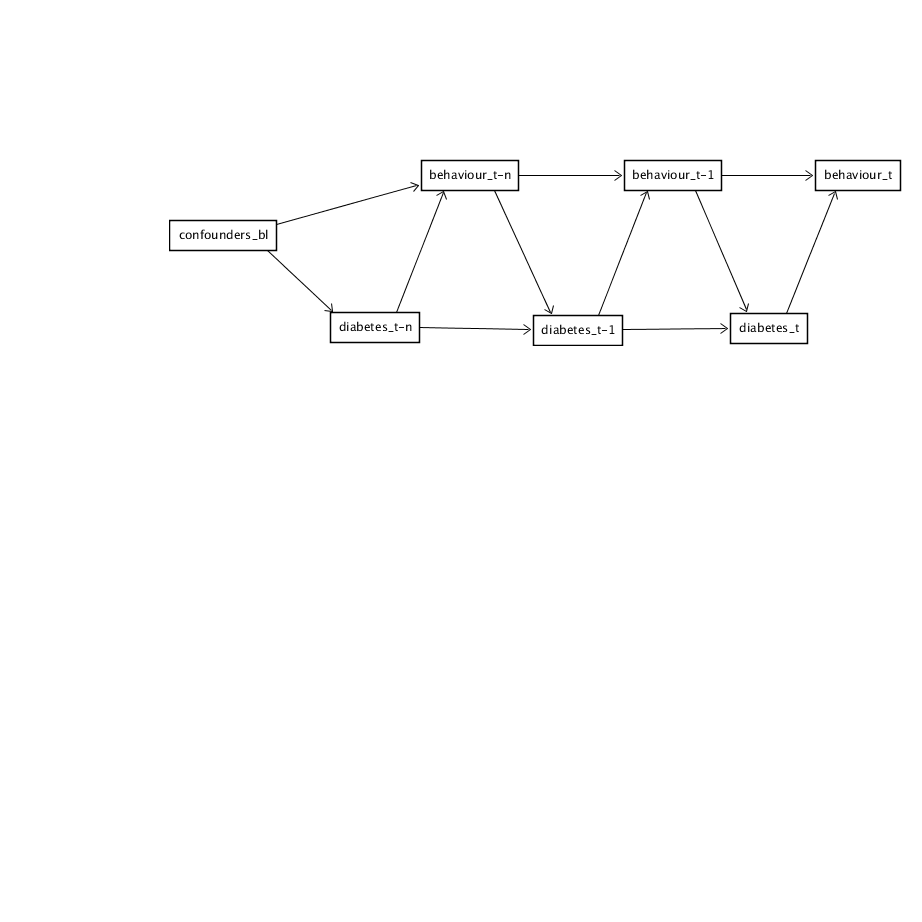
\includegraphics[scale=0.7]{Chapter5/Figures/dag}
\end{center}
\footnotesize{\textit{Notes} The confounders not only include control variables but also pre-treatment values of our outcomes of interest to account for any predetermination of the treatment.}

\end{figure}


In our context it seems possible that, for example, \ac{BMI} could affect the probability of being diagnosed with diabetes which then itself may affect subsequent \ac{BMI} levels, confounding the relationship between a diabetes diagnosis and \ac{BMI} due to non-random selection. Similarly, employment history and current employment could affect the probability of a diabetes diagnosis through their impact on lifestyle and hence diabetes risk factors such as increases weight or smoking. For example, an increase in disposable income or a reduction in leisure time as a result of a new job and the subsequent effect on risk behaviours could confound the relationship between a diabetes diagnosis and employment status. \ac{MSM} accounts for this by calculating weights based on the potential risk of a person being diagnosed at each time point. 

To calculate these weights we first construct unstabilized weights using baseline values of time-variant confounders, time-invariant confounders as well as time-variant confounders lagged by one period to predict the probability of developing diabetes at each wave. We use lagged time-variant confounders because current diabetes status as reported in the survey was determined at some point within the current and the previous wave that were determined before the current diabetes status, to prevent reverse causality. The used predictors are age and age squared to account for changes in risk with increasing age, an index of urbanization pre-constructed within the \ac{CHNS} data, ranging from 1 to 120 as the level of urbanization increases \parencite{Zhang2014d}, to account for the impact of urbanization on diabetes risk \parencite{Attard2012}. We also use secondary and university education, being married, having any medical insurance, being of Han ethnicity, living in a rural area, dummies for the different Chinese regions and the respective survey waves as predictors. Further we use inflation adjusted per-capita household income to adjust for effects of household wealth on diabetes. Finally, all outcome variables (employment status, alcohol consumption, smoking status, \ac{BMI}, waist circumference and average daily calorie consumption) are used as predictors. 

Because unstabilized weights can be highly variable it is recommended to stabilize the weights \parencite{Cole2008}. Using the unstabilized weights as the denominator, stabilized weights are calculated by dividing the denominator by the predicted treatment propensity from a model using only time-invariant confounders and baseline information of the time-variant confounders as predictors.  Because our analysis is stratified by males and females, we create weights separately for both groups.

The \acp{MSM} are estimated using \ac{OLS} for the continuous and a logistic model for the binary outcomes. For the logistic model we calculate average marginal effects for greater comparability with the results of the \ac{FE} models. All models are weighted by the stabilized weights constructed beforehand while adjusting for all baseline and time-invariant covariates used in the calculation of the stabilized weights, except for the respective outcome of interest. Robust standard errors to account for intra-class correlation of repeated outcome measurements in individuals are used throughout. In our primary analysis, we present the results of the \ac{MSM} with untruncated stabilized weights, as these provide theoretically unbiased estimates, albeit they likely are less efficient than truncated weights \parencite{Cole2008}. The distribution of the inverse probability weights supports this decision as there are no extreme values and the mean weight is 1 (see Table \ref{tab:stabweights}).

\subsubsection*{Fixed effects}

While the \ac{MSM} can account for pre-treatment selection on observable and time-variant confounders, it assumes that there are no unobserved time-invariant confounders such as family background, cognitive abilities, and other personal characteristics. This is a strong assumption that may be violated. The individual level \ac{FE} model can help remedy this problem as it is able to account for both observed time-variant and invariant variables as well as time-invariant unobserved variables. It does so by demeaning the confounding variables at each time point by the overall individual mean across all observed time points. It then uses solely the within-person variation for identification, thereby accounting for any time-invariant observed or unobserved as well as observed time-variant effects. 

This comes at a price: due to the demeaning, time-invariant variables such as Han ethnicity, are dropped from the model and cannot not be estimated. Further, because the \ac{FE} model is not able to account for any treatment effects on other time-variant confounders, only a more limited set of confounders could be included compared to the \ac{MSM}. Otherwise our estimate of the effect of a diabetes diagnosis would likely be biased due to the inclusion of 'bad controls' \parencite{Angrist2009a}. Bad controls are those that have been affected by the treatment itself---such as \ac{BMI} or smoking status after a diabetes diagnosis---and therefore likely capture part of the causal effect of diabetes on our outcome of interest, biasing the diabetes coefficient \parencite{Angrist2009a}. The \ac{FE} models thus only includes controls for age, age squared, the level of urbanization, education, being married, having any medical insurance, living in a rural area, and dummies for the different Chinese regions and the respective survey waves. For the estimation of the effect of time since diagnosis, the linear age variable is dropped. In \ac{FE} models, two or more variables that change at the same rate between waves cannot be separately identified. Here this is the case with age and time-dummies, as both variables increase by one each additional year \parencite{Wooldridge2012}. To identify the effect of diabetes duration we have to rely on the presence of people without diabetes in the sample, for which diabetes duration does not increase at the same rate as time.

Because it is not possible to retrieve marginal effects from a logistic \ac{FE} model, we use a \ac{FE} linear probability model instead. It generally produces very similar estimates compared to non-linear models \parencite{Angrist2009a}.

\subsubsection*{Multiple imputation}

To deal with missing data, we used chained multiple imputation to impute the missing values in Stata 13 using the user written ICE command \parencite{Royston2009} and used the resulting data for all our estimated models. Overall, thirty imputed datasets were created. Imputation models included all variables used in the \acp{MSM}. We imputed missing data in the same wave for which some data were recorded; we did not impute completely missing waves. Further, we did not impute missing diabetes information and instead assumed that once a diabetes diagnosis was reported, the individual had diabetes in every ensuing wave, even when the observation was missing. If diabetes was never reported in any wave, we assumed that the individual never had diabetes. We then only imputed missing values for those observations that had a non-missing diabetes status. For the calculation of the marginal effects in the \ac{MSM} logit models, Rubin's rules were applied using the user written Stata command mimrgns \parencite{Klein2014}.

\subsubsection*{Numbers of observations}

Because we used lagged variables to construct the stabilized weights for the \acp{MSM}, the number of observations used in the \acp{MSM} was lower than those used in the \ac{FE} models, where we did not use lagged variables. The summary statistics shown in Table \ref{tab:descriptives_diab} are based on the observations used in the \ac{FE} models.

\subsubsection*{Sensitivity analyses}

We conduct three additional sensitivity analyses in order to test the robustness of our results to different assumptions and estimation strategies.
First, we estimate all models using only covariate adjustment in a \ac{RE} model, to investigate in how far this 'naive' approach diverts from the "causal" estimates of the \ac{FE} and \acp{MSM}. These results are presented and discussed together with the \ac{MSM} and \ac{FE} results. Second, we truncate weights at the 1\textsuperscript{st} and 99\textsuperscript{th} percentile to investigate the sensitivity of the \acp{MSM} to the most extreme weights. While untruncated weights provide unbiased estimates under the assumptions of the \ac{MSM}, they may not be the most efficient and tend to have larger standard errors \parencite{Cole2008}. Third, we estimate the \ac{FE} and \acp{MSM} using the original non-imputed data to ascertain the extent to which multiple imputation affected the results.

\section{\label{sec:Results5}Results}

From the descriptive statistics, we can observe that people with diabetes in any wave are less likely to be employed. Looking at health behaviours, it is mainly men that smoke and report alcohol consumption while very few women do so. The prevalence of smoking and drinking was lower for men with diabetes; they also consumed fewer calories compared to men without diabetes. Further, the diabetes group has both higher \ac{BMI} and waist circumference levels. They are also older, live in more urbanized areas, are more likely to have insurance and men are somewhat better educated while women are less educated compared to their counterparts without diabetes. Both men and women report an average time since diagnosis of around 4.5 years. Looking at per capita household income, men and women with diabetes come from household with higher income levels than those without a diabetes diagnosis. Further it appears that in China it is less educated women that report a diagnosis, while men with diabetes are better educated compared to those without diabetes.

\begin{landscape}
\begin{table}[p]
\caption{\label{tab:descriptives_diab}Sample means for males and females, by diabetes status}
\begin{center}
\begin{adjustbox}{max width=\linewidth}  
{
\def\sym#1{\ifmmode^{#1}\else\(^{#1}\)\fi}
\begin{tabular}{l*{6}{SS}}
\toprule
                    &\multicolumn{3}{c}{Males}             &\multicolumn{3}{c}{Females}           \\\cmidrule(lr){2-4}\cmidrule(lr){5-7}
                    &\multicolumn{1}{c}{No diabetes}&\multicolumn{1}{c}{Diabetes}&\multicolumn{1}{c}{p-value (t-test)}&\multicolumn{1}{c}{No diabetes}&\multicolumn{1}{c}{Diabetes}&\multicolumn{1}{c}{p-value (t-test)}\\
\midrule
Employed            &        82\%&        68\%&    <0.001        &        67\%&        29\%&     <0.001       \\
Smokes              &        58\%&        47\%&      <0.001      &        3\%&        4\%&    0.409        \\
Any alcohol consumption&     63\%&        53\%&       <0.001     &        9\%&        4\%&   <0.001         \\
Daily Kcal eaten (3-day average)&     2422&     2166&      <0.001      &     2068&     1931&   0.001         \\
BMI                 &       22.99&      24.90&       <0.001     &       23.10&       25.80&    <0.001        \\
Waist circ. (cm)    &       82.02&       88.81&      <0.001      &       78.80&       87.55&     <0.001       \\
Age                 &       42.27&      52.76&      <0.001      &       43.24&       55.32&     <0.001       \\
Han ethnicity       &        87\%&      89\%&     0.292       &        87\%&        93\%&     0.002      \\
Rural area          &        69\%&       52\%&     <0.001       &        68\%&        51\%&     <0.001       \\
Married             &        83\%&      93\%&     <0.001       &        88\%&        87\%&    0.392        \\
Secondary education     &        65\%&      68\%&   0.439         &        50\%&        43\%&       0.007     \\
University education    &        5\%&      11\%&    <0.001        &        4\%&        1\%&     0.017      \\
Any health insurance&        51\%&     82\%&     <0.001       &        50\%&        71\%&       <0.001      \\
Urbanization Index  &       60.87&     74.48&     <0.001       &       61.77&       68.68&     <0.001       \\
Per capita household income (Yuan (2011))&    8617&     16328&    <0.001        &     8581&     11101&    <0.001        \\
Years since diabetes diagnosis&       -&        4.5&      -      &        -&        4.65&      -      \\
\midrule
Observations        &       23413&         284&       23697&       23577&         336&       23913     \\
\bottomrule
\end{tabular}
}
\end{adjustbox}
\end{center}
\end{table}
\end{landscape}
\FloatBarrier

Predicting the denominator for the stabilized weights we find that for men a higher baseline \ac{BMI} increases the risk of a diabetes diagnosis. Further, increases in age, waist circumference as well as urbanization levels are associated with higher chances for men to be diagnosed with diabetes throughout the survey. Interestingly becoming employed may decrease the chances of being diagnosed with diabetes slightly, justifying the use of the \ac{MSM} in our employment models as well  (Table \ref{tab:predictors}). Because these are not causal estimates, it may be that it is more likely for men with a lower risk of diabetes to select into employment. Interestingly, we do not find that higher household income levels are predictive of a diagnosis for men or women, despite what the descriptive statistics indicated. For women, higher age at baseline, increases in \ac{BMI} and waist circumference  as well as living in a non-rural environment predict a diabetes diagnosis.

\begin{table}[p]
\caption{\label{tab:predictors}Time variant and invariant predictors of a diabetes diagnosis  (denominator of stabilized weights)}
\begin{center}
\begin{adjustbox}{max width=\linewidth}  
{
\def\sym#1{\ifmmode^{#1}\else\(^{#1}\)\fi}
\begin{tabular}{l*{4}{S S}}
\toprule
                &\multicolumn{2}{c}{Males}&\multicolumn{2}{c}{Females}\\\cmidrule(lr){2-3}\cmidrule(lr){4-5}&\multicolumn{1}{c}{(1)}&\multicolumn{1}{c}{(2)}&\multicolumn{1}{c}{(3)}&\multicolumn{1}{c}{(4)}\\
                &\multicolumn{1}{c}{$\beta$}&\multicolumn{1}{c}{SE}&\multicolumn{1}{c}{$\beta$}&\multicolumn{1}{c}{SE}\\
\midrule
Age (bl)          &-.000 &.001         &.004\sym{**} & .002         \\
Age squared (bl)       &.000 &.000         &-.000\sym{**} &.000         \\
\ac{BMI} (bl)        &.001\sym{***} &.000         &.001 &.000         \\
Waist circumference (cm) (bl)        &.000 &.000         &.000\sym{*} &.000         \\
3-Day Ave: Energy (kcal) (bl)       &-.000 &.000         &.000 &.000         \\
Smoking (bl)    &.001 &.002         &.003 &.006         \\
Alcohol consumption (bl)        &.003\sym{*} &.002         &.000 &.005         \\
Urbanization index (bl)      &-.000 &.000         &-.000 & .000         \\
Secondary educ. (bl)    &-.001 &.003         &.003 &.003         \\
University educ. (bl) &-.000 &.006         & -         \\
Married (bl)      &-.002 &.004         &-.000 &.004         \\
Any medical insurance (bl)    &.002 &.002         &-.000 &.002         \\
Employed (bl)        &.002 &.003         &.001 &.002         \\
Han ethnicity   &.001 &.003         &-.002 &.003         \\
Rural      &-.001 &.002         &-.005\sym{***} &.002         \\
Per capita household income (2011 Yuan) (bl)&-.000 &.000         &-.000 &.000         \\
Survey year && \\
\hspace*{10mm}2004&.002 &.002         &-.001 &.002         \\
\hspace*{10mm}2006&.003 &.002         &-.003 &.003         \\
\hspace*{10mm}2009&.009\sym{***} &.003         &-.001 &.004         \\
\hspace*{10mm}2011&.001 &.003         &.001 &.004         \\
Age           &.003\sym{**} &.001         &-.002 &.002         \\
Age squared        &-.000\sym{**} &.001         &.000 &.000         \\
BMI          &-.001 &.000        &.001\sym{**} &.000         \\
Waist circumference (cm)         &.000 &.000         &-.000 &.000         \\
3-Day Ave: Energy (kcal)        &-.000 &.000         &-.000 &.000         \\
Smoking         &-.003 &.002         &.000 &.006         \\
Alcohol consumption        &-.004\sym{**} &.002         &-.003 &.006         \\
Urbanization index         &.000 &.000         &.000 &.000         \\
Secondary education     &.001 &.003         &.000 &.003         \\
University education    &.001 &.006         & -         \\
Married       &-.000 &.004         &-.003 &.004         \\
Any medical insurance     &.001 &.002         &-.001 &.002         \\
Employed         &-.004\sym{**} &.002         &-.003 &.002         \\
Per capita household income (2011 Yuan) (2011 Yuan) &.000 &.000         &-.000 &.000         \\
\bottomrule
\multicolumn{5}{l}{\footnotesize \sym{*} \(p<0.10\), \sym{**} \(p<0.05\), \sym{***} \(p<0.01\)}\\
\multicolumn{5}{l}{\footnotesize Results for province dummies omitted to preserve space. No observations for women with university education and diabetes.}\\
\end{tabular}
}
\end{adjustbox}
\end{center}
\end{table}

The results of our regression analysis are presented in Table \ref{tab:binary}. Both the \ac{FE} model and the \ac{MSM} indicate that women with a diabetes diagnosis have reduced probabilities of being employed than their counterparts without diabetes, with a reduction of 11 percentage points in the \ac{FE} model and 12 percentage points in the \ac{MSM}. This translates into a relative reduction in employment probabilities between 16--17\%. For men no such effect is observed.

\begin{table}[p]

\caption{\label{tab:binary}Analysis of the effect of a diabetes diagnosis on employment status and behavioural outcomes using fixed effects and marginal structural models}
\begin{adjustbox}{max width=\linewidth, center}
\begin{threeparttable}  %adds notes to tables
{
\def\sym#1{\ifmmode^{#1}\else\(^{#1}\)\fi}
\begin{tabular}{l*{6}{S
S}}
\toprule
                &\multicolumn{1}{c}{(1)}&\multicolumn{1}{c}{(2)}&\multicolumn{1}{c}{(3)}&\multicolumn{1}{c}{(4)}&\multicolumn{1}{c}{(5)}&\multicolumn{1}{c}{(6)}\\
                &\multicolumn{1}{c}{Employment}&\multicolumn{1}{c}{Smoking}&\multicolumn{1}{c}{Alcohol}&\multicolumn{1}{c}{BMI}&\multicolumn{1}{c}{Waist (cm)}&\multicolumn{1}{c}{Calories (kcal)}\\
                \midrule
&\multicolumn{6}{c}{\emph{Marginal structural model}} \\  
\addlinespace                                   

Male sample &&&&&&\\
Diabetes&      -.009         &    -.070\sym{**} &    -.094\sym{***}&    -.735\sym{***}&   -1.887\sym{***}& -135.061\sym{**} \\
                &   (.026)         &   (.032)         &   (.036)         &   (.180)         &   (.574)         & (58.593)         \\
Female sample &&&&&&\\
Diabetes     &     -.117\sym{***}&    -.015\sym{*}  &    -.029\sym{**} &    -.388         &    -.335         &  -45.630         \\
                &   (.029)         &   (.008)         &   (.012)         &   (.240)         &   (.631)         & (33.530)         \\    
\midrule      
\addlinespace 
&\multicolumn{6}{c}{\emph{Fixed effects}} \\
\addlinespace             
Male sample &&&&&&\\
Diabetes        &      .022         &    -.023         &    -.104\sym{***}&    -.715\sym{***}&   -2.217\sym{***}& -168.297\sym{***}\\
                &   (.030)         &   (.032)         &   (.036)         &   (.183)         &   (.610)         & (62.115)         \\
Female sample &&&&&&\\
Diabetes        &    -.112\sym{***}&    -.027\sym{**} &    -.012         &    -.644\sym{**} &   -1.251\sym{**} &  -61.175         \\
                &   (.035)         &   (.013)         &   (.010)         &   (.263)         &   (.616)         & (47.420)         \\ 
\midrule      
\addlinespace                 
&\multicolumn{6}{c}{\emph{Random effects}} \\
\addlinespace             
Male sample &&&&&&\\
Diabetes        &    -.022         &    -.064\sym{**} &    -.104\sym{***}&    -.379\sym{**} &    -.756         & -172.467\sym{***}\\
                &   (.028)         &   (.029)         &   (.029)         &   (.177)         &   (.542)         & (48.768)         \\
Female sample &&&&&&\\
Diabetes        &    -.152\sym{***}&    -.021\sym{**} &    -.019\sym{***}&    -.263         &     .459         &  -39.267         \\
                &   (.027)         &   (.011)         &   (.006)         &   (.247)         &   (.570)         & (34.256)         \\                            
\bottomrule
\end{tabular}
\begin{tablenotes}
\item \textit{Notes} Standard errors in parentheses. Other control variables: age (only MSM), age squared, region, urban, education, han, marital status, urbanization index, time dummies, health insurance status, per capite household income.  Fixed/random effects: N=23443 (male sample), N=23702 (female sample); MSM:  N=16047 (male sample), N=16658 (female sample).
\item \sym{*} \(p<0.10\), \sym{**} \(p<0.05\), \sym{***} \(p<0.01\))
\end{tablenotes}
}
\end{threeparttable}
\end{adjustbox}

\end{table}

There is a more ambiguous picture for the effect of a diabetes diagnosis on behavioural outcomes. There is no consistent---and only marginally significant evidence in the \ac{MSM}---that men reduced their smoking rate, however, a diabetes diagnosis led to a reduction in alcohol consumption as according to either model, though particularly so for the \ac{MSM}. For waist circumference, \ac{BMI} and calorie consumption, the \ac{FE} and \ac{MSM} both indicate reductions in \ac{BMI} of close to 0.7, of about 2 cm in waist circumference and of up to 170 calories per day for men. Results for women look different, in that while the point estimates indicate a reduction in all outcomes, these tend to be smaller than those for men and only exhibit strong statistical significance in the \ac{FE} model for \ac{BMI}, waist circumference and alcohol consumption.

The results of the \ac{RE} models appear to overestimate the impact of diabetes on female employment probabilities and to underestimate the impact of a diabetes diagnosis on reductions in \ac{BMI} and waist circumference. For the other outcomes, results are very similar to those from the \acp{MSM} and \ac{FE} models.

Exploring the effect of a diabetes diagnosis over time, we first estimated a specification using time since diagnosis as a continuous variable. The results of the \ac{FE} model (Table \ref{tab:duration}) indicate a steady reduction of female employment probabilities of almost two percentage points per year and of male alcohol consumption, \ac{BMI}, waist circumference and consumed calories. The \ac{MSM} again supports the finding of the \ac{FE} model, finding very similar effects in terms of size and statistical significance. For women, the \ac{MSM} also support the finding of a reduction in employment probabilities, with the point estimate  being somewhat larger compared to the \ac{FE} model. The evidence for changes in health behaviours is less consistent across models and outcomes, with the \ac{FE} indicating a reduction in waist circumference but not in \ac{BMI}, and the \ac{MSM} suggesting the opposite. The effect sizes for changes in health behaviours in women are about half the size to those found in men. 

The results of the \ac{RE} models again likely overestimate the impact of diabetes on female employment probabilities and to underestimate the impact of a diabetes diagnosis on reductions in \ac{BMI} and waist circumference. 


\begin{table}[p]
\caption{\label{tab:duration}Analysis of the effect of time since diabetes diagnosis on employment status and behavioural outcomes using fixed effects and marginal structural models}
\begin{adjustbox}{max width=\linewidth} 
\begin{threeparttable}  %adds notes to tables
{
\def\sym#1{\ifmmode^{#1}\else\(^{#1}\)\fi}
\begin{tabular}{l*{6}{S S}} \toprule
                &\multicolumn{3}{c}{Odds ratios}                   &\multicolumn{3}{c}{Beta coefficients}         \\\cmidrule(lr){2-4}\cmidrule(lr){5-7}
                &\multicolumn{1}{c}{(1)}&\multicolumn{1}{c}{(2)}&\multicolumn{1}{c}{(3)}&\multicolumn{1}{c}{(4)}&\multicolumn{1}{c}{(5)}&\multicolumn{1}{c}{(6)}\\
                &\multicolumn{1}{c}{Employment}&\multicolumn{1}{c}{Smoking}&\multicolumn{1}{c}{Any alcohol}&\multicolumn{1}{c}{\ac{BMI}}&\multicolumn{1}{c}{Waist (cm)}&\multicolumn{1}{c}{Calories (kcal)}\\
                \midrule
&\multicolumn{6}{c}{\emph{Marginal structural model}} \\
\addlinespace                     
Male sample &&&&&&\\
Time since diagnosis&    -.003         &    -.010\sym{*}  &    -.014\sym{**} &    -.127\sym{***}&    -.340\sym{***}&  -21.770\sym{**} \\
                &   (.004)         &   (.005)         &   (.007)         &   (.031)         &   (.099)         &  (9.842)         \\
Female sample &&&&&&\\
Time since diagnosis&      -.017\sym{***}&    -.002         &    -.004         &    -.066\sym{*}  &    -.072         &   -8.735         \\
                &   (.005)         &   (.001)         &   (.003)         &   (.040)         &   (.109)         &  (5.589)         \\
\addlinespace 
\midrule
&\multicolumn{6}{c}{\emph{Fixed effects}} \\               
\addlinespace
Male sample &&&&&&\\
Time since diagnosis   &  -.001         &    -.003         &    -.017\sym{**} &    -.150\sym{***}&    -.520\sym{***}&  -22.286\sym{**} \\
                &   (.007)         &   (.006)         &   (.007)         &   (.037)         &   (.121)         & (11.083)         \\
Female sample &&&&&&\\
Time since diagnosis  & -.019\sym{***}&    -.003         &    -.000         &    -.102\sym{***}&    -.215\sym{*}  &   -6.747         \\
                &   (.007)         &   (.002)         &   (.001)         &   (.039)         &   (.117)         &  (7.028)         \\                 
\midrule      
\addlinespace                 
&\multicolumn{6}{c}{\emph{Random effects}} \\
\addlinespace             
Male sample &&&&&&\\
Diabetes        &    -.006         &    -.009\sym{*}  &    -.015\sym{***}&    -.099\sym{***}&    -.269\sym{***}&  -24.703\sym{***}\\
                &   (.006)         &   (.006)         &   (.005)         &   (.035)         &   (.096)         &  (8.655)         \\
Female sample &&&&&&\\
Diabetes        &     -.023\sym{***}&    -.002         &    -.002\sym{**} &    -.056         &     .013         &   -6.444         \\
                &   (.006)         &   (.002)         &   (.001)         &   (.039)         &   (.114)         &  (5.670)         \\ 
\bottomrule
\end{tabular}
\begin{tablenotes}
\item \textit{Notes} Standard errors in parentheses. Other control variables: age (only MSM), age squared, region, urban, education, han, marital status, urbanization index, time dummies, health insurance status, household expenditures. Fixed/random effects: N=23443 (male sample), N=23702 (female sample); MSM:  N=16047 (male sample), N=16658 (female sample)
\item \sym{*} \(p<0.10\), \sym{**} \(p<0.05\), \sym{***} \(p<0.01\))
\end{tablenotes}
}
\end{threeparttable}
\end{adjustbox}
\end{table}

\FloatBarrier

In a second step we estimated a specification using year dummies to capture the potential non-linearity in the relationship between time since diagnosis and our outcomes. The results for both estimation methods are visualized in Figure \ref{fig:duration_g_fe_mi} and presented in Tables \ref{tab:duration_groups_fe} and \ref{tab:duration_groups_msm} for the \ac{FE} and \ac{MSM}, respectively. Despite the smaller sample size in each group and hence lower precision, the \ac{FE} model still indicates a reduction in \ac{BMI} and waist circumference for men, especially in the first 8 to 10 years after diagnosis. A similar effect is found for females, especially for years 3 to 8 after diagnosis. Interestingly, female employment already decreases rapidly in the first to second year after diagnosis and it does not appear that females are able to increase their employment probabilities later on. Using the \ac{MSM}, all point estimates suggest similar effects, but due to the lower sample size, we were not able to estimate the effects for females on smoking and alcohol consumption.


\begin{figure}
\begin{center}
\caption{\label{fig:duration_g_fe_mi} Analysis of the effect of time since diabetes diagnosis on employment status and behavioural outcomes (duration groups)}
Marginal structural models
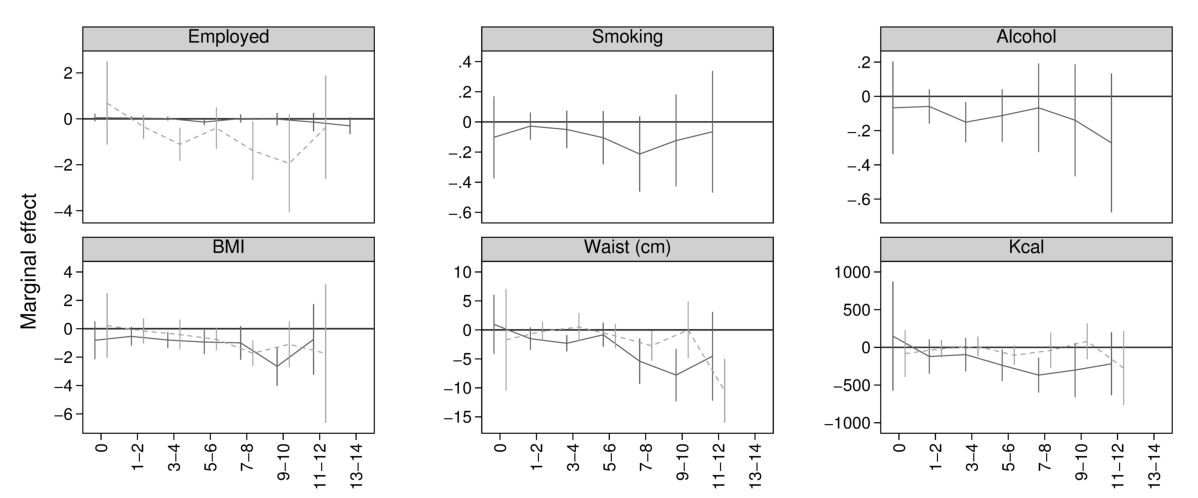
\includegraphics[width=\linewidth]{Chapter5/Figures/mi_msm_l_all1.pdf}
Fixed effects
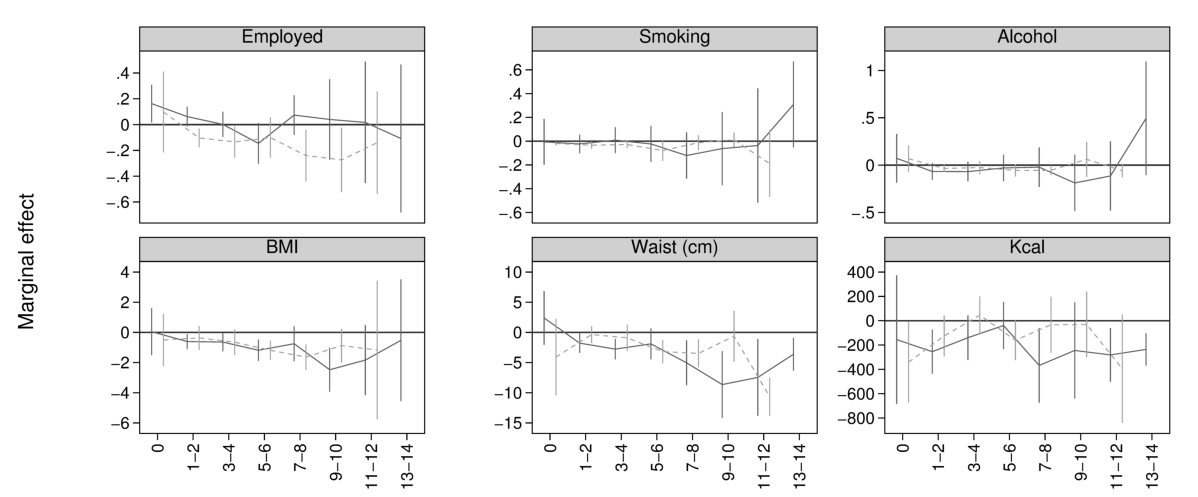
\includegraphics[width=\linewidth]{Chapter5/Figures/mi_fe2.pdf}
Random effects
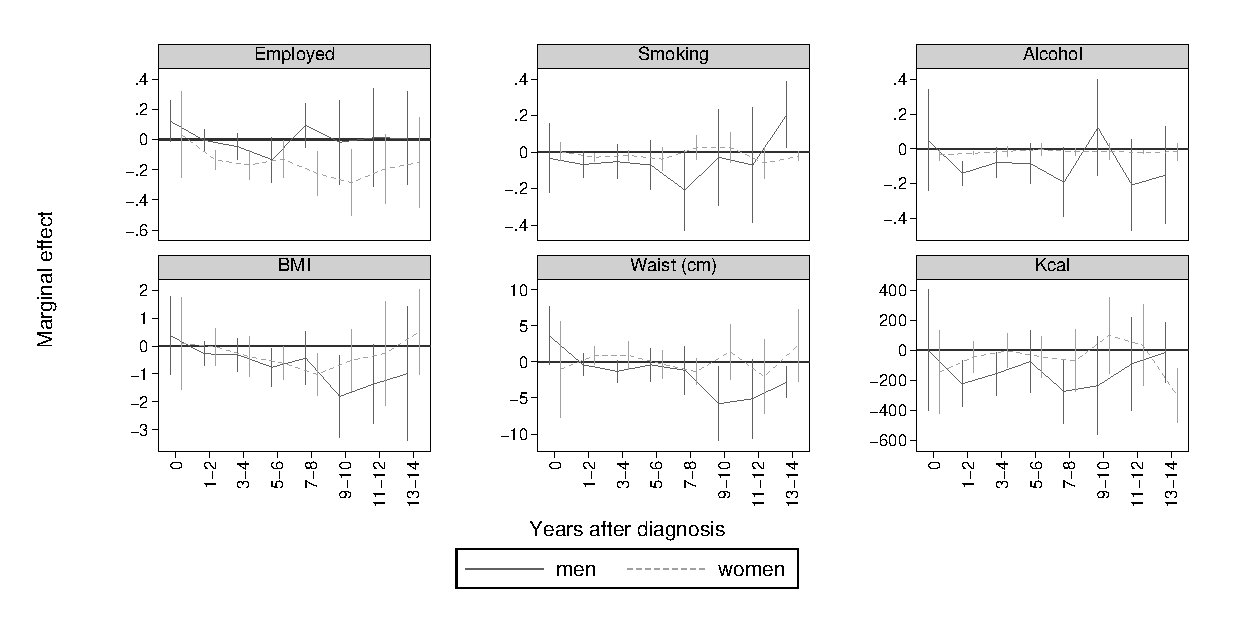
\includegraphics[width=\linewidth]{Chapter5/Figures/mi_re}
\end{center}
\end{figure}


We conducted two sensitivity analyses. First, we truncated weights at the 1\textsuperscript{st} and 99\textsuperscript{th} percentile to investigate the sensitivity of the \acp{MSM} to the most extreme weights. The estimated effects are very similar to those using the untruncated weights (Table \ref{tab:truncation} and \ref{tab:duration_groups_tr}), suggesting no important loss in efficiency and supporting the decision to use untruncated weights. Second, we estimated the \ac{FE} and \acp{MSM} using the original non-imputed data. The results are broadly similar (Tables \ref{tab:binary_non_mi}, \ref{tab:duration_non_mi}, \ref{tab:duration_groups_non_mi_fe} and \ref{tab:duration_groups_non_mi_msm}), in particular for the \ac{FE} model, still indicating a reduction in female employment chances and male alcohol consumption, \ac{BMI} and waist circumference. The coefficients of the \ac{MSM} still point into the same direction as those using the imputed data, but the estimated effects are smaller in size and confidence intervals are relatively large.


\FloatBarrier


\section{\label{sec:Discussion5}Disussion}

Our results suggest that receiving a diabetes diagnosis in China led to a strong and lasting reduction in female, but not male employment probabilities. Looking at the behavioural risk factor outcomes, \ac{BMI} and waist circumference as well as risk behaviours such as alcohol and calorie consumption and potentially smoking were found to be reduced for men. For females, our primary results did not find as strong indications for changes in behavioural risk factors. Accordingly, it appears that women in China have to endure stronger adverse labour market effects and at the same time are less successful then men at making risk behaviour changes to reduce their risk of diabetes complications.

The \ac{MSM} models and \ac{FE} models indicated very similar results suggesting that they are robust and that time-invariant confounding factors may play a limited role over and above baseline and time varying confounding factors. The \ac{MSM} results suggest that in particular high baseline \ac{BMI} and waist circumference levels help explain selection into a diabetes diagnosis, and thus need to be taken into account. Further, becoming employed appears to decrease the risk of being diagnosed with diabetes. The robustness checks using 'naive' regression in the form of \ac{RE} models further indicated that in this setting insufficiently accounting for confounding leads to an overestimation of the impact of diabetes on employment status and an underestimation of the effects of a diagnosis on weight measures (\ac{BMI} and waist circumference). However, confounding may only be of limited relevance after adjusting for observable covariates for risk behaviours (smoking and alcohol consumption) and caloric intake.

\subsection{Limitations}

While we used two estimation methods to reduce the influence of selection bias due to unobserved confounding, one limitation of the used approaches is their inability to account for all forms of selection simultaneously. Therefore a causal interpretation is only possible under restrictive assumptions, namely no unobserved time-variant confounding for the \ac{FE} model and positivity, exchangeability and consistency for the \ac{MSM}. The assumption of positivity is likely to hold, given that every person should have at least a small chance of receiving a diabetes diagnosis. This is also supported by the relatively small range of stabilized weights and absence of zero-weights. Exchangeability, or no unmeasured confounding, is not testable and could potentially be violated if not all time-invariant or time-variant confounders were accounted for. We tested for part of this assumption by estimating a \ac{FE} model, which suggested that unobserved time-invariant confounding may be of limited relevance. Consistency would have been violated if a diabetes diagnosis had been reported but the person had actually not been diagnosed with diabetes. This is likely only violated in very rare cases of misreporting, given that specificity of diabetes self-report is very high in China \autocite{Yuan2015}. Because we were interested in the effect of a diabetes diagnosis, unobserved diabetes did not violate the consistency assumption.

A limitation of the \ac{FE} model is the possibility of time-variant confounding causing selection into a diabetes diagnosis based on changes in pre-treatment values of our outcomes of interest. Given that the \ac{FE} estimates were close to those of the \acp{MSM}, it is likely that there was no strong confounding due to pre-treatment changes. Rather, the similarity of results suggests that it is important to account for some form of baseline values, be it via demeaning as in the \ac{FE} model or by using baseline values in the \ac{MSM}.  Further, the \ac{FE} model is unable to account for the effect of confounders that are causally related with diabetes such as \ac{BMI} or waist circumference but may also have an effect on the outcome themselves. This may lead to an over- or underestimation of the effect of diabetes if the diabetes variable captures parts of the effect of very high \ac{BMI} levels (obesity). This may be the reason for some of the, albeit small, differences in point estimates between the \ac{FE} model and \ac{MSM}.

Finally, an important limitation is the that a diabetes diagnosis entails a variety of 'treatments' that are difficult to disentangle and may each have a distinct effect on the explored outcomes. Currently, we are only able to observe the combined effect of these treatments. Firstly, there is the provision of information at diagnosis, potentially causing increases in stress and anxiety, but may also providing an explanation for the experienced symptoms, both potentially affecting productivity. Secondly, a diagnosis also is the starting point for medical treatment, potentially alleviating symptoms and helping with weight loss, but also posing new challenges, in particular if treatment entails the exogenous provision of insulin or strict meal plans, potentially adding to the burden of diabetes in daily life. Thirdly, adherence to medical treatment may be heterogeneous across people with diabetes, with non-adherence likely leading to a further worsening of risk factors for complications, while good adherence may be able to prevent or delay debilitating complications. Fourthly, a diagnosis may also introduces lifestyle changes such as increasing exercise levels, eating healthier and reducing smoking or alcohol consumption, all potentially affecting the risk to develop further complications and to experience changes in productivity. In the current study, it is not possible to ascertain which of these factors and to what extend are affecting employment chances, but also the observed changes in weight loss. Only for the reductions in smoking and alcohol consumption, it seems reasonable to attribute them to diagnosis induced awareness to reduce these risk factors.


\subsection{Potential mechanisms}

The permanent reduction in male \ac{BMI} and waist circumference we have found has also been observed in a cohort of Danish patients \autocite{DeFineOlivarius2015}, where weight increased the years preceding diagnosis, while after diagnosis weight decreased. The exact reasons for this decrease were unknown but attributed to motivation changes as a result of the diagnosis, concluding that time around the diagnosis may represent a window of opportunity to obtain long lasting weight change. Nonetheless, reductions in weight, as already eluded to in the limitations, may also be the result of treatment initiation with metformin or other diabetes drugs that have been shown to lead to weight reductions \autocite{Yang2014}. Importantly, the reduction in \ac{BMI} in our study was accompanied by a reduction in waist circumference and energy intake.  Given that in China diabetes incidence has been especially attributed to a high accumulation of visceral fat and central obesity \autocite{Ma2014}, reductions in waist circumference therefore may have a particular positive effect on diabetes control and the prevention of comorbidities. This also allows for the interpretation  that the changes in \ac{BMI} are due to reductions in fat and not lean body mass\autocite{Klein2007}. The reduction in energy intake further suggest that the changes in weight are at least partly the result of changes in food consumption.

For women, however, we did not find similar strong evidence for reductions in \ac{BMI}, waist circumference or energy intake. The relatively smaller effects for women could indicate a lower ability to change behaviours supportive of weight loss. This appears to be supported by the smaller reductions in energy intake. This could have---at least partly---contributed to a higher risk for further diabetes complications that then reduced employment probabilities. Apart from this, other explanations for the lower weight loss and larger employment penalty for women compared to men include their lower educational attainment, which has been indicated as a factor in preventing better glucose control \autocite{Luo2015} and may also affect the ability to successfully change behaviours. Lower income levels for females compared to men may also negatively affect the ability to receive adequate treatment following a diagnosis, limiting their ability to change health behaviours \autocite{Luo2015} and increasing the risk of complications. We found that women with diabetes lived in households with lower income levels compared to men with diabetes, however, these income levels were still higher then for those without diabetes. Nonetheless, it may still be the case that women are able to use fewer household revenues for their own healthcare. Further, there are likely biological factors that lead to worse health outcomes for women compared to men. There is some evidence that, due to different ways of fat storage between men and women, men tend to cross the diabetes threshold at an earlier point in time and at a comparatively healthier metabolic state then women \parencite{Peters2015,Peters2014a,Peters2014}. Women are more likely to have spend more time in a pre-diabetes stadium \parencite{Bertram2010} and to cross the threshold only once the metabolic has significantly deteriorated, leading to a greater risk of cardiovascular disease and stroke \parencite{Peters2015}. Supporting this, a study for China found a greater prevalence of diabetes comorbidities in Chinese women than men \autocite{Liu2010}. In this light it may not be surprising that we find more conclusive evidence of worsening employment probabilities for women than for men. If women are less likely to receive proper treatment and to change their health behaviours and at the same time have a greater risk for complications then men, the long term effects of diabetes on their health are likely more severe than for men and consequently affect their employment status.

The found adverse effect of diabetes on employment is in line with other studies on the labour market impact of diabetes that find adverse effects of diabetes on women employment probabilities \parencite{Minor2010,Latif2009,Harris2009,Seuring2016}---often stronger than the effects experienced by men. Most comparable, due to the use of \ac{FE} with data for a similar time period, a study from Mexico also found significant reductions for both males and females of about 5 percentage points \parencite{Seuring2016}. Taking into account the lower overall employment rate of Mexican women compared to men, this translated into an about 16\% reduction in employment probabilities, a figure comparable to what Chinese women experienced. However, in Mexico also men experienced adverse effects, unlike to what we found for China.

The found effects on changes in behavioural risk factors can partly be compared to a study by \parencite{Slade2012} that used population level observational data to investigate the effect of a diabetes diagnosis on health behaviours in the USA. Our findings are similar in some respects, as both studies suggest a response to the diabetes diagnosis 'shock' by reductions in dietary choices---Slade also found a reduction in alcohol consumption---but not to a similar extend curb smoking. In terms of the effect on weight, both studies cannot be directly compared because Slade investigated the effect to be overweight or obese, while we used continuous weight measures due to the discussed difficulties of defining cut-off values for Asian populations. Nonetheless, the results from the overweight and obesity models we estimated do---similarly to Slade---not indicate important reductions in obesity after a diabetes diagnosis. However, while Slade finds a stronger initial reduction in weight status, he also finds that people with diabetes tended to return to be obese or overweight after some time. Our results suggested that man may manage to consistently reduce their probabilities to be obese, but not overweight, at least according to the \ac{FE} model. Importantly---and in concordance with our findings---he finds that simple covariate adjustment leads to estimates indicating an increase in overweight and obesity, underlining the importance of accounting for unobserved heterogeneity.



\section{Conclusion}

Our results indicate changes in male health behaviours after a diabetes diagnosis in China. These findings are robust to the application of two distinct, but complementary econometric techniques. Further, women likely had to bear a larger diabetes burden also affecting their economic well-being, as evidenced by their reduction in employment probabilities. Potentially, one of the causes of these adverse economic effects is the lower ability of women to successfully change their behaviour as a result of the diagnosis. Further research should try to unravel the mechanisms behind these differential outcomes for men and women. Overall, given the large prevalence of undiagnosed diabetes, our results indicate that an early diagnosis may be a good way to foster early behaviour change that could lead to more positive health and economic outcomes for people with diabetes over time. It appears, however, that more emphasis on the adequate treatment options for women may be needed to reduce their burden of diabetes. 

\clearpage

\subsection*{Stabilized weights}

\begin{table}[p]
\caption{\label{tab:stabweights}Summary of stabilized weights}
\begin{adjustbox}{max width=\linewidth}  
{
\def\sym#1{\ifmmode^{#1}\else\(^{#1}\)\fi}
\begin{tabular}{l*{1}{ccc}}
\toprule
                    &        Mean&         Min&         Max\\
\midrule
Untruncated (men)   &    1.001343&    .1740716&   5.780513\\
Untruncated (women) &    1.000773&   .1661002&  8.754402\\
Truncated 1 and 99 percentile (men)&    .9997768&    .8906016&    1.107517\\
Truncated 1 and 99 percentile (women)&    .9988097&    .8323757&    1.119154\\
\end{tabular}
}
\end{adjustbox}
\end{table}

\FloatBarrier

\clearpage
\subsection{Duration groups results}


\begin{table}[p]
\caption{\label{tab:duration_groups_msm}Analysis of the effect of time since diabetes diagnosis on employment status and behavioural outcomes using marginal structural models (duration groups)}
\begin{adjustbox}{max width=\linewidth}  
\begin{threeparttable}
{
\def\sym#1{\ifmmode^{#1}\else\(^{#1}\)\fi}
\begin{tabular}{l*{6}{S
S}}
\toprule
                &\multicolumn{1}{c}{(1)}&\multicolumn{1}{c}{(2)}&\multicolumn{1}{c}{(3)}&\multicolumn{1}{c}{(4)}&\multicolumn{1}{c}{(5)}&\multicolumn{1}{c}{(6)}\\
                &\multicolumn{1}{c}{Employment}&\multicolumn{1}{c}{Smoking}&\multicolumn{1}{c}{Any alcohol}&\multicolumn{1}{c}{BMI}&\multicolumn{1}{c}{Waist (cm)}&\multicolumn{1}{c}{Calories (kcal)}\\
\midrule
\addlinespace                                   
Male sample &&&&&&\\
0               &     .049         &    -.102         &    -.067         &    -.811         &     .968         &  148.433         \\
                &   (.087)         &   (.139)         &   (.138)         &   (.682)         &  (2.587)         &(369.013)         \\
\addlinespace
1-2             &     .034         &    -.028         &    -.059         &    -.535         &   -1.517         & -121.424         \\
                &   (.038)         &   (.046)         &   (.051)         &   (.340)         &   (.996)         &(115.615)         \\
\addlinespace
3-4             &     .012         &    -.050         &    -.150\sym{**} &    -.795\sym{***}&   -2.312\sym{***}&  -96.393         \\
                &   (.042)         &   (.063)         &   (.060)         &   (.288)         &   (.712)         &(113.071)         \\
\addlinespace
5-6             &    -.139\sym{**} &    -.105         &    -.112         &    -.937\sym{**} &    -.843         & -237.957\sym{**} \\
                &   (.068)         &   (.090)         &   (.078)         &   (.438)         &  (1.050)         &(107.745)         \\
\addlinespace
7-8             &     .010         &    -.213\sym{*}  &    -.067         &    -.995\sym{*}  &   -5.401\sym{***}& -368.463\sym{***}\\
                &   (.087)         &   (.127)         &   (.132)         &   (.602)         &  (1.991)         &(117.513)         \\
\addlinespace
9-10            &    -.014         &    -.124         &    -.139         &   -2.648\sym{***}&   -7.791\sym{***}& -300.917         \\
                &   (.136)         &   (.155)         &   (.167)         &   (.699)         &  (2.294)         &(184.269)         \\
\addlinespace
11-12           &    -.142         &    -.065         &    -.272         &    -.751         &   -4.542         & -218.570         \\
                &   (.203)         &   (.205)         &   (.206)         &  (1.262)         &  (3.896)         &(212.524)         \\
\addlinespace
13-14           &    -.304         &                  &                  &                  &                  &                  \\
                &   (.186)         &                  &                  &                  &                  &                  \\
\midrule
Female sample &&&&&&\\
0               &     .110         &         &         &     .233         &   -1.713         &  -82.792         \\
                &   (.132)         &         &         &  (1.158)         &  (4.483)         &(158.560)         \\
\addlinespace
1-2             &    -.063         &         &         &    -.153         &    -.238         &  -17.870         \\
                &   (.049)         &         &         &   (.450)         &   (.850)         & (59.249)         \\
\addlinespace
3-4             &    -.210\sym{***}&         &         &    -.409         &     .506         &   11.054         \\
                &   (.071)         &         &         &   (.537)         &  (1.229)         & (67.419)         \\
\addlinespace
5-6             &    -.074         &         &         &    -.743\sym{*}  &   -1.038         & -104.696         \\
                &   (.087)         &         &         &   (.396)         &  (1.063)         & (64.981)         \\
\addlinespace
7-8             &    -.262\sym{**} &         &         &   -1.721\sym{***}&   -2.724\sym{**} &  -41.099         \\
                &   (.122)         &         &         &   (.464)         &  (1.315)         &(119.484)         \\
\addlinespace
9-10            &    -.355\sym{**} &         &         &   -1.095         &    -.012         &   80.030         \\
                &   (.172)         &         &         &   (.827)         &  (2.495)         &(122.037)         \\
\addlinespace
11-12           &    -.072         &         &         &   -1.739         &  -10.515\sym{***}& -275.508         \\
                &   (.213)         &         &         &  (2.489)         &  (2.806)         &(250.141)         \\
\bottomrule
\end{tabular}
\begin{tablenotes}
\item \textit{Notes} Other control variables: age, age squared, region, urban, education, han, marital status, urbanization index, time dummies, health insurance status, household expenditures. N=13195 (male sample), N=14549 (female sample).
\item \sym{*} \(p<0.10\), \sym{**} \(p<0.05\), \sym{***} \(p<0.01\))
\end{tablenotes}
}
\end{threeparttable}
\end{adjustbox}
\end{table}
\clearpage

\begin{table}[p]
\caption{\label{tab:duration_groups_fe}Analysis of the effect of time since diabetes diagnosis on employment status and behavioural outcomes using fixed effects (duration groups)}
\begin{adjustbox}{max width=\linewidth} 
\begin{threeparttable} 
{
\def\sym#1{\ifmmode^{#1}\else\(^{#1}\)\fi}
\begin{tabular}{l*{6}{S S}} \toprule
                &\multicolumn{3}{c}{Odds ratios}                   &\multicolumn{3}{c}{Beta coefficients}         \\\cmidrule(lr){2-4}\cmidrule(lr){5-7}
                &\multicolumn{1}{c}{(1)}&\multicolumn{1}{c}{(2)}&\multicolumn{1}{c}{(3)}&\multicolumn{1}{c}{(4)}&\multicolumn{1}{c}{(5)}&\multicolumn{1}{c}{(6)}\\
                &\multicolumn{1}{c}{Employment}&\multicolumn{1}{c}{Smoking}&\multicolumn{1}{c}{Any alcohol}&\multicolumn{1}{c}{\ac{BMI}}&\multicolumn{1}{c}{Waist (cm)}&\multicolumn{1}{c}{Calories (kcal)}\\
                \midrule            
Male sample &&&&&&\\
0               &     .163\sym{**} &    -.006         &     .072         &     .049         &    2.397         & -155.323         \\
                &   (.075)         &   (.098)         &   (.132)         &   (.792)         &  (2.258)         &(268.552)         \\
\addlinespace
1-2             &     .062         &    -.023         &    -.067         &    -.605\sym{**} &   -1.782\sym{**} & -254.427\sym{***}\\
                &   (.039)         &   (.040)         &   (.045)         &   (.252)         &   (.825)         & (92.421)         \\
\addlinespace
3-4             &     .002         &     .008         &    -.068         &    -.639\sym{**} &   -2.768\sym{***}& -139.397         \\
                &   (.050)         &   (.055)         &   (.052)         &   (.314)         &   (.870)         & (93.516)         \\
\addlinespace
5-6             &    -.145\sym{*}  &    -.023         &    -.030         &   -1.183\sym{***}&   -1.901         &  -39.053         \\
                &   (.081)         &   (.077)         &   (.071)         &   (.362)         &  (1.304)         & (98.730)         \\
\addlinespace
7-8             &     .074         &    -.121         &    -.021         &    -.751         &   -5.037\sym{***}& -367.421\sym{**} \\
                &   (.079)         &   (.100)         &   (.106)         &   (.588)         &  (1.896)         &(156.656)         \\
\addlinespace
9-10            &     .040         &    -.062         &    -.188         &   -2.472\sym{***}&   -8.642\sym{***}& -244.372         \\
                &   (.159)         &   (.157)         &   (.152)         &   (.741)         &  (2.812)         &(201.960)         \\
\addlinespace
11-12           &     .017         &    -.037         &    -.114         &   -1.835         &   -7.465\sym{**} & -281.008\sym{**} \\
                &   (.240)         &   (.245)         &   (.187)         &  (1.181)         &  (3.238)         &(112.461)         \\
\addlinespace
13-14           &    -.108         &     .308\sym{*}  &     .494         &    -.524         &   -3.615\sym{***}& -235.985\sym{***}\\
                &   (.293)         &   (.184)         &   (.306)         &  (2.059)         &  (1.383)         & (67.961)         \\
\midrule
Female sample &&&&&&\\
0               &     .098         &    -.019\sym{**} &     .067         &    -.505         &   -4.090         & -340.952\sym{**} \\
                &   (.159)         &   (.008)         &   (.072)         &   (.896)         &  (3.235)         &(169.411)         \\
\addlinespace
1-2             &    -.103\sym{***}&    -.034\sym{**} &    -.036\sym{*}  &    -.364         &    -.355         & -124.847         \\
                &   (.037)         &   (.015)         &   (.020)         &   (.404)         &   (.717)         & (85.402)         \\
\addlinespace
3-4             &    -.134\sym{**} &    -.028\sym{*}  &    -.025         &    -.648         &    -.896         &   45.970         \\
                &   (.062)         &   (.016)         &   (.036)         &   (.435)         &  (1.120)         & (79.063)         \\
\addlinespace
5-6             &    -.100         &    -.079\sym{*}  &    -.056\sym{*}  &   -1.184\sym{***}&   -3.176\sym{***}& -160.445\sym{*}  \\
                &   (.080)         &   (.045)         &   (.033)         &   (.323)         &   (.990)         & (83.164)         \\
\addlinespace
7-8             &    -.240\sym{**} &    -.013         &    -.054\sym{**} &   -1.637\sym{***}&   -3.482\sym{***}&  -32.865         \\
                &   (.103)         &   (.032)         &   (.026)         &   (.433)         &  (1.182)         &(117.750)         \\
\addlinespace
9-10            &    -.274\sym{**} &     .012         &     .062         &    -.876         &    -.639         &  -30.676         \\
                &   (.128)         &   (.031)         &   (.094)         &   (.568)         &  (2.147)         &(137.658)         \\
\addlinespace
11-12           &    -.140         &    -.189         &    -.059         &   -1.163         &  -10.633\sym{***}& -393.884\sym{*}  \\
                &   (.202)         &   (.143)         &   (.036)         &  (2.344)         &  (1.618)         &(227.502)         \\     
\bottomrule
\end{tabular}
\begin{tablenotes}
\item \textit{Notes} Other control variables: age squared, region, urban, education, han, marital status, urbanization index, time dummies, health insurance status, household expenditures. N=13195 (male sample), N=14549 (female sample).
\item \sym{*} \(p<0.10\), \sym{**} \(p<0.05\), \sym{***} \(p<0.01\))
\end{tablenotes}
}
\end{threeparttable}
\end{adjustbox}
\end{table}
\FloatBarrier

\clearpage
\subsection*{Robustness checks}

\subsubsection*{\acp{MSM} using truncated weights}
\begin{table}[p]
\caption{\label{tab:truncation}Analysis of the effect of a diabetes diagnosis on employment status and behavioural outcomes using marginal structural models with truncated stabilized weights at 1st and 99th percentile}
\begin{adjustbox}{max width=\linewidth}  
\begin{threeparttable}
{
\def\sym#1{\ifmmode^{#1}\else\(^{#1}\)\fi}
\begin{tabular}{l*{6}{S
S}}
\toprule
                &\multicolumn{1}{c}{(1)}&\multicolumn{1}{c}{(2)}&\multicolumn{1}{c}{(3)}&\multicolumn{1}{c}{(4)}&\multicolumn{1}{c}{(5)}&\multicolumn{1}{c}{(6)}\\
                &\multicolumn{1}{c}{Employment}&\multicolumn{1}{c}{Smoking}&\multicolumn{1}{c}{Any alcohol}&\multicolumn{1}{c}{BMI}&\multicolumn{1}{c}{Waist (cm)}&\multicolumn{1}{c}{Calories (kcal)}\\
\midrule
&\multicolumn{6}{c}{\emph{Diabetes}} \\
\addlinespace    
Male sample &&&&&& \\
Diabetes&   -.022         &    -.070\sym{**} &    -.094\sym{***}&    -.732\sym{***}&   -1.637\sym{***}& -175.662\sym{***}\\
                &   (.023)         &   (.032)         &   (.036)         &   (.179)         &   (.532)         & (51.574)         \\
Female sample &&&&&& \\
Diabetes&    -.132\sym{***}&    -.015\sym{*}  &    -.029\sym{**} &    -.178         &     .186         &  -47.980         \\
                &   (.029)         &   (.008)         &   (.012)         &   (.248)         &   (.638)         & (34.319)         \\   
\addlinespace 
\midrule
&\multicolumn{6}{c}{\emph{Years since diagnosis}} \\               
\addlinespace  
Male sample &&&&&&\\
Time since diagnosis     &    -.006         &    -.010\sym{**} &    -.016\sym{**} &    -.133\sym{***}&    -.326\sym{***}&  -26.261\sym{***}\\
                &   (.004)         &   (.005)         &   (.006)         &   (.033)         &   (.095)         &  (9.160)         \\

Female sample &&&&&&\\
Time since diagnosis&  -.019\sym{***}&    -.002         &    -.004         &    -.044         &    -.016         &   -9.096         \\
                &   (.006)         &   (.001)         &   (.003)         &   (.042)         &   (.112)         &  (5.681)         \\          
\bottomrule
\end{tabular}
\begin{tablenotes}
\item \textit{Notes}   Standard errors in parentheses.
Other control variables: age squared, region, urban, education, han, marital status, urbanization index, time dummies, health insurance status, household expenditures. N=16047 (male sample), N=16658 (female sample).
\end{tablenotes}
}
\end{threeparttable}
\end{adjustbox}
\end{table}

\clearpage

\begin{table}[p]
\caption{\label{tab:duration_groups_tr}Effect of time since diabetes diagnosis on employment status and behavioural outcomes using MSM with truncated stabilized weights (1st and 99th pct; imputed)}
\begin{adjustbox}{max width=\linewidth}  
\begin{threeparttable}
{
\def\sym#1{\ifmmode^{#1}\else\(^{#1}\)\fi}
\begin{tabular}{l*{6}{S
S}}
\toprule
                &\multicolumn{1}{c}{(1)}&\multicolumn{1}{c}{(2)}&\multicolumn{1}{c}{(3)}&\multicolumn{1}{c}{(4)}&\multicolumn{1}{c}{(5)}&\multicolumn{1}{c}{(6)}\\
                &\multicolumn{1}{c}{Employment}&\multicolumn{1}{c}{Smoking}&\multicolumn{1}{c}{Any alcohol}&\multicolumn{1}{c}{BMI}&\multicolumn{1}{c}{Waist (cm)}&\multicolumn{1}{c}{Calories (kcal)}\\
\midrule       
Male sample &&&&&&\\
0               &     .075         &    -.102         &    -.067         &    -.345         &    2.302         &  -86.368         \\
                &   (.077)         &   (.139)         &   (.138)         &   (.839)         &  (2.872)         &(247.229)         \\
\addlinespace
1-2             &     .012         &    -.028         &    -.059         &    -.375         &    -.812         & -224.716\sym{**} \\
                &   (.036)         &   (.046)         &   (.051)         &   (.297)         &   (.957)         & (95.028)         \\
\addlinespace
3-4             &    -.018         &    -.050         &    -.150\sym{**} &    -.723\sym{**} &   -1.965\sym{***}& -167.769\sym{*}  \\
                &   (.042)         &   (.063)         &   (.060)         &   (.305)         &   (.735)         & (86.996)         \\
\addlinespace
5-6             &    -.139\sym{**} &    -.105         &    -.112         &   -1.034\sym{***}&    -.891         & -203.814\sym{**} \\
                &   (.066)         &   (.090)         &   (.078)         &   (.392)         &  (1.096)         &(102.051)         \\
\addlinespace
7-8             &     .018         &    -.213\sym{*}  &    -.067         &    -.944\sym{*}  &   -4.935\sym{***}& -347.441\sym{***}\\
                &   (.084)         &   (.127)         &   (.132)         &   (.563)         &  (1.846)         &(125.660)         \\
\addlinespace
9-10            &    -.033         &    -.124         &    -.139         &   -2.627\sym{***}&   -6.998\sym{***}& -232.656         \\
                &   (.122)         &   (.155)         &   (.167)         &   (.689)         &  (2.453)         &(177.019)         \\
\addlinespace
11-12           &    -.151         &    -.065         &    -.272         &    -.889         &   -4.363         & -212.318         \\
                &   (.202)         &   (.205)         &   (.206)         &  (1.123)         &  (3.500)         &(189.967)         \\
\addlinespace
13-14           &    -.305\sym{*}  &                  &                  &                  &                  &                  \\
                &   (.185)         &                  &                  &                  &                  &                  \\
\midrule
Female sample &&&&&&\\
0               &     .112         &         &         &     .685         &    -.060         & -104.652         \\
                &   (.128)         &         &         &  (1.289)         &  (4.993)         &(158.546)         \\
\addlinespace
1-2             &    -.104\sym{**} &         &         &     .205         &     .698         &  -18.334         \\
                &   (.047)         &         &         &   (.452)         &   (.834)         & (64.456)         \\
\addlinespace
3-4             &    -.208\sym{***}&         &         &    -.299         &     .889         &    6.982         \\
                &   (.068)         &         &         &   (.520)         &  (1.191)         & (65.213)         \\
\addlinespace
5-6             &    -.138\sym{*}  &         &         &    -.569         &    -.793         & -122.064\sym{*}  \\
                &   (.082)         &         &         &   (.364)         &  (1.087)         & (64.349)         \\
\addlinespace
7-8             &    -.249\sym{**} &         &         &   -1.662\sym{***}&   -2.125         &   -5.039         \\
                &   (.121)         &         &         &   (.502)         &  (1.315)         &(120.139)         \\
\addlinespace
9-10            &    -.373\sym{**} &         &         &   -1.019         &     .409         &   72.475         \\
                &   (.169)         &         &         &   (.829)         &  (2.523)         &(132.027)         \\
\addlinespace
11-12           &    -.087         &         &         &   -1.858         &  -10.814\sym{***}& -251.975         \\
                &   (.214)         &         &         &  (2.510)         &  (2.749)         &(234.610)         \\
\bottomrule
\end{tabular}
\begin{tablenotes}
\item \textit{Notes}   Standard errors in parentheses.
Other control variables: age squared, region, urban, education, Han, marital status, urbanization index, time dummies, health insurance status, household expenditures. N=13195 (male sample), N=14549 (female sample).
\end{tablenotes}
}
\end{threeparttable}
\end{adjustbox}
\end{table}

\FloatBarrier
\clearpage
\subsubsection*{Results using non-imputed data}

\begin{table}[p]
\caption{\label{tab:binary_non_mi}Analysis of the effect of a diabetes diagnosis on employment status and behavioural outcomes using fixed effects and marginal structural models (no imputation)}
\begin{adjustbox}{max width=\linewidth, center}
\begin{threeparttable}
{
\def\sym#1{\ifmmode^{#1}\else\(^{#1}\)\fi}
\begin{tabular}{l*{6}{S
S}}
\toprule
                &\multicolumn{1}{c}{(1)}&\multicolumn{1}{c}{(2)}&\multicolumn{1}{c}{(3)}&\multicolumn{1}{c}{(4)}&\multicolumn{1}{c}{(5)}&\multicolumn{1}{c}{(6)}\\
                &\multicolumn{1}{c}{Employment}&\multicolumn{1}{c}{Smoking}&\multicolumn{1}{c}{Any alcohol}&\multicolumn{1}{c}{BMI}&\multicolumn{1}{c}{Waist (cm)}&\multicolumn{1}{c}{Calories (kcal)}\\
\midrule
&\multicolumn{6}{c}{\emph{Marginal structural model}} \\
\addlinespace             
Male sample &&&&&&\\
Diabetes&          .050         &    -.042         &    -.112\sym{**} &    -.641\sym{***}&   -1.224         & -152.149         \\
                &   (.046)         &   (.041)         &   (.049)         &   (.220)         &   (.803)         &(123.921)         \\
Female sample &&&&&&\\
Diabetes&            -.081\sym{*}  &    -.028\sym{*}  &    -.075         &    -.583         &    -.935         &  -50.350         \\
                &   (.049)         &   (.015)         &   (.045)         &   (.393)         &   (.866)         & (56.914)         \\
\addlinespace 
\midrule
&\multicolumn{6}{c}{\emph{Fixed effects}} \\  
\addlinespace                                   
Male sample &&&&&&\\
Diabetes&        .028         &    -.000         &    -.063\sym{*}  &    -.868\sym{***}&   -2.448\sym{***}& -152.027\sym{**} \\
                &   (.030)         &   (.033)         &   (.034)         &   (.170)         &   (.517)         & (68.421)         \\
Female sample &&&&&&\\
Diabetes&         -.107\sym{***}&    -.024\sym{**} &    -.022         &    -.638\sym{**} &   -1.049\sym{*}  &  -81.554\sym{*}  \\
                &   (.034)         &   (.012)         &   (.019)         &   (.288)         &   (.636)         & (48.970)         \\                                      
\bottomrule
\end{tabular}
\begin{tablenotes}
\item \textit{Notes}   Standard errors in parentheses.
Other control variables: age (only MSM), age squared, region, urban, education, han, marital status, urbanization index, time dummies, health insurance status, household expenditures. FE:  N=21444 (male sample), N=23128 (female sample), MSM: N=10039 (male sample), N=11489 (female sample).
\end{tablenotes}
}
\end{threeparttable}
\end{adjustbox}
\end{table}

\clearpage

\begin{table}[p]
\caption{\label{tab:duration_non_mi}Analysis of the effect of time since diabetes diagnosis on employment status and behavioural outcomes using fixed effects and marginal structural models (non-imputed)}
\begin{adjustbox}{max width=\linewidth}  
\begin{threeparttable}
{
\def\sym#1{\ifmmode^{#1}\else\(^{#1}\)\fi}
\begin{tabular}{l*{6}{SS}}
\toprule
                &\multicolumn{1}{c}{(1)}&\multicolumn{1}{c}{(2)}&\multicolumn{1}{c}{(3)}&\multicolumn{1}{c}{(4)}&\multicolumn{1}{c}{(5)}&\multicolumn{1}{c}{(6)}\\
                &\multicolumn{1}{c}{Employment}&\multicolumn{1}{c}{Smoking}&\multicolumn{1}{c}{Any alcohol}&\multicolumn{1}{c}{BMI}&\multicolumn{1}{c}{Waist (cm)}&\multicolumn{1}{c}{Calories (kcal)}\\
                \midrule
&\multicolumn{6}{c}{\emph{Marginal structural model}} \\               
\addlinespace 
Male sample &&&&&&\\
Time since diagnosis&   .027         &    -.020         &    -.024         &    -.221\sym{**} &    -.705\sym{**} &  -80.594\sym{**} \\
                &   (.018)         &   (.016)         &   (.017)         &   (.087)         &   (.295)         & (39.681)         \\
Female sample &&&&&&\\
Time since diagnosis&    -.030         &    -.009         &    -.039         &    -.413\sym{*}  &    -.598         &  -14.552         \\
                &   (.022)         &   (.006)         &   (.025)         &   (.216)         &   (.376)         & (24.269)         \\ 
\addlinespace 
\midrule      
&\multicolumn{6}{c}{\emph{Fixed effects}} \\
\addlinespace                     
Male sample &&&&&&\\
Time since diagnosis&  -.003         &     .005         &    -.003         &    -.164\sym{***}&    -.581\sym{***}&  -22.700         \\
                &   (.008)         &   (.007)         &   (.007)         &   (.044)         &   (.121)         & (12.487)         \\
Female sample &&&&&&\\
Time since diagnosis&    -.026\sym{**} &    -.006\sym{*}  &    -.005         &    -.163\sym{**} &    -.325\sym{*}  &  -16.888         \\
                &   (.009)         &   (.002)         &   (.004)         &   (.060)         &   (.148)         & (10.337)         \\                          
\bottomrule
\end{tabular}
\begin{tablenotes}
\item \textit{Notes}   Standard errors in parentheses.
Other control variables: age (only MSM) age squared, region, urban, education, han, marital status, urbanization index, time dummies, health insurance status, household expenditures. FE:  N=22066 (male sample), N=23051 (female sample), MSM: N=10028 (male sample), N=11465 (female sample).
\end{tablenotes}
}
\end{threeparttable}
\end{adjustbox}
\end{table}

\clearpage


\begin{table}[p]
\caption{\label{tab:duration_groups_non_mi_msm}Analysis of the effect of time since diabetes diagnosis on employment status and behavioural outcomes using marginal structural models (duration groups) (non-imputed)}
\begin{adjustbox}{max width=\linewidth}  
\begin{threeparttable}
{
\def\sym#1{\ifmmode^{#1}\else\(^{#1}\)\fi}
\begin{tabular}{l*{6}{SS}}
\toprule
                &\multicolumn{1}{c}{(1)}&\multicolumn{1}{c}{(2)}&\multicolumn{1}{c}{(3)}&\multicolumn{1}{c}{(4)}&\multicolumn{1}{c}{(5)}&\multicolumn{1}{c}{(6)}\\
                &\multicolumn{1}{c}{Employment}&\multicolumn{1}{c}{Smoking}&\multicolumn{1}{c}{Any alcohol}&\multicolumn{1}{c}{BMI}&\multicolumn{1}{c}{Waist (cm)}&\multicolumn{1}{c}{Calories (kcal)}\\
\midrule          
Male sample &&&&&&\\
0               &     .107         &     .051         &    -.149         &   -1.004\sym{*}  &    1.113         &  314.866         \\
                &   (.080)         &   (.150)         &   (.175)         &   (.562)         &  (1.103)         &(409.370)         \\
\addlinespace
1-2             &     .038         &    -.050         &    -.050         &    -.609\sym{**} &   -1.727\sym{*}  & -146.884         \\
                &   (.047)         &   (.052)         &   (.057)         &   (.284)         &   (.973)         &(148.251)         \\
\addlinespace
3-4             &     .000         &    -.038         &    -.095         &   -1.028\sym{**} &   -3.164         & -695.698\sym{***}\\
                &      (.)         &   (.159)         &   (.117)         &   (.460)         &  (2.066)         &(190.065)         \\
\midrule
Female sample &&&&&&\\
0               &     .134         &     .000         &     .000         &    -.102         &   -1.362         & -111.379         \\
                &   (.179)         &      (.)         &      (.)         &  (1.544)         &  (6.099)         &(207.839)         \\
\addlinespace
1-2             &    -.079         &    -.019\sym{**} &    -.052\sym{*}  &    -.484         &    -.581         &  -32.105         \\
                &   (.069)         &   (.008)         &   (.029)         &   (.487)         &  (1.006)         & (67.670)         \\
\addlinespace
3-4             &     .000         &     .000         &     .000         &   -5.590\sym{*}  &   -8.485\sym{***}&    1.258         \\
                &      (.)         &      (.)         &      (.)         &  (3.286)         &  (1.792)         &(258.264)         \\      
\bottomrule
\end{tabular}
\begin{tablenotes}
\item \textit{Notes} Due to    Standard errors in parentheses.
Other control variables: Age, age squared, region, urban, education, han, marital status, urbanization index, time dummies, health insurance status, household expenditures.    N=10028 (male sample), N=11465 (female sample).
\end{tablenotes}
}
\end{threeparttable}
\end{adjustbox}
\end{table}

\clearpage

\begin{table}[p]
\caption{\label{tab:duration_groups_non_mi_fe}Analysis of the effect of time since diabetes diagnosis on employment status and behavioural outcomes using fixed effects (duration groups) (non-imputed)}
\begin{adjustbox}{max width=\linewidth}  
\begin{threeparttable}
{
\def\sym#1{\ifmmode^{#1}\else\(^{#1}\)\fi}
\begin{tabular}{l*{6}{SS}}
\toprule
                &\multicolumn{1}{c}{(1)}&\multicolumn{1}{c}{(2)}&\multicolumn{1}{c}{(3)}&\multicolumn{1}{c}{(4)}&\multicolumn{1}{c}{(5)}&\multicolumn{1}{c}{(6)}\\
                &\multicolumn{1}{c}{Employment}&\multicolumn{1}{c}{Smoking}&\multicolumn{1}{c}{Any alcohol}&\multicolumn{1}{c}{BMI}&\multicolumn{1}{c}{Waist (cm)}&\multicolumn{1}{c}{Calories (kcal)}\\
\midrule
Male sample &&&&&&\\
0               &     .132         &    -.014         &     .125         &    -.009         &    1.439         & -268.692         \\
                &   (.072)         &   (.085)         &   (.136)         &   (.702)         &  (1.879)         &(215.527)         \\
\addlinespace
1-2             &     .065         &    -.013         &    -.053         &    -.849\sym{***}&   -2.391\sym{***}& -244.075\sym{**} \\
                &   (.039)         &   (.041)         &   (.045)         &   (.212)         &   (.663)         & (91.888)         \\
\addlinespace
3-4             &     .009         &     .058         &    -.035         &    -.720\sym{*}  &   -2.642\sym{**} & -105.039         \\
                &   (.048)         &   (.054)         &   (.053)         &   (.334)         &   (.824)         &(100.459)         \\
\addlinespace
5-6             &    -.127         &     .029         &    -.006         &   -1.168\sym{***}&   -1.733         &  -14.828         \\
                &   (.080)         &   (.079)         &   (.078)         &   (.351)         &  (1.204)         &(104.926)         \\
\addlinespace
7-8             &     .118         &    -.089         &     .030         &    -.617         &   -4.227\sym{*}  & -319.563         \\
                &   (.081)         &   (.090)         &   (.087)         &   (.537)         &  (1.871)         &(166.278)         \\
\addlinespace
9-10            &     .018         &     .030         &    -.115         &   -2.199\sym{***}&   -9.351\sym{***}& -189.090         \\
                &   (.154)         &   (.132)         &   (.145)         &   (.659)         &  (2.503)         &(224.518)         \\
\addlinespace
11-12           &    -.032         &     .097         &     .058         &   -2.060         &   -9.185\sym{**} & -162.422         \\
                &   (.250)         &   (.200)         &   (.097)         &  (1.074)         &  (2.868)         & (94.541)         \\
\addlinespace
13-14           &    -.116         &     .341\sym{*}  &     .599         &    -.527         &   -3.481\sym{***}& -146.776\sym{*}  \\
                &   (.312)         &   (.153)         &   (.311)         &  (1.959)         &   (.864)         & (68.253)         \\
\midrule
Female sample &&&&&&\\
0               &     .117         &    -.019\sym{*}  &     .066         &    -.811         &   -4.079         & -372.137\sym{*}  \\
                &   (.154)         &   (.008)         &   (.072)         &   (.912)         &  (3.403)         &(171.871)         \\
\addlinespace
1-2             &    -.091\sym{*}  &    -.032\sym{*}  &    -.037         &    -.324         &    -.383         & -133.764\sym{*}  \\
                &   (.037)         &   (.014)         &   (.021)         &   (.417)         &   (.681)         & (61.475)         \\
\addlinespace
3-4             &    -.144\sym{*}  &    -.024         &    -.025         &    -.857         &   -1.051         &   26.559         \\
                &   (.061)         &   (.014)         &   (.039)         &   (.458)         &  (1.184)         & (85.752)         \\
\addlinespace
5-6             &    -.118         &    -.080         &    -.062\sym{*}  &   -1.243\sym{***}&   -2.531\sym{**} & -190.484\sym{*}  \\
                &   (.080)         &   (.046)         &   (.031)         &   (.348)         &   (.958)         & (94.117)         \\
\addlinespace
7-8             &    -.255\sym{*}  &     .004         &    -.050         &   -1.823\sym{***}&   -3.976\sym{**} &  -47.473         \\
                &   (.102)         &   (.020)         &   (.026)         &   (.454)         &  (1.217)         &(133.625)         \\
\addlinespace
9-10            &    -.249\sym{*}  &     .016         &     .064         &   -1.121         &    -.803         &  -89.938         \\
                &   (.125)         &   (.033)         &   (.102)         &   (.653)         &  (2.277)         &(136.611)         \\
\addlinespace
11-12           &    -.197         &    -.224         &    -.069         &    -.878         &  -10.898\sym{***}& -563.138\sym{*}  \\
                &   (.170)         &   (.172)         &   (.041)         &  (2.888)         &  (1.724)         &(240.085)         \\      
\bottomrule
\end{tabular}
\begin{tablenotes}
\item \textit{Notes}   Standard errors in parentheses.
Other control variables: age squared, region, urban, education, han, marital status, urbanization index, time dummies, health insurance status, household expenditures. N=22066 (male sample), N=23051 (female sample).
\end{tablenotes}
}
\end{threeparttable}
\end{adjustbox}
\end{table}

\FloatBarrier
\clearpage




\subsection*{Overweight and obesity results}

\begin{table}[p]
\caption{\label{tab:obesity_FE}Analysis of the effect of a diabetes diagnosis on overweight and obesity}
\begin{adjustbox}{max width=\linewidth, center}  
\begin{threeparttable}
{
\def\sym#1{\ifmmode^{#1}\else\(^{#1}\)\fi}
\begin{tabular}{l*{4}{S
S}}
\toprule
                &\multicolumn{2}{c}{Males}            &\multicolumn{2}{c}{Females}          \\\cmidrule(lr){2-3}\cmidrule(lr){4-5}
                &\multicolumn{1}{c}{(1)}&\multicolumn{1}{c}{(2)}&\multicolumn{1}{c}{(3)}&\multicolumn{1}{c}{(4)}\\
                &\multicolumn{1}{c}{Overweight}&\multicolumn{1}{c}{Obese}&\multicolumn{1}{c}{Overweight}&\multicolumn{1}{c}{Obese}\\
                \midrule
&\multicolumn{4}{c}{\emph{Marginal structural model}} \\               
\addlinespace   
Diabetes& -.000         &    -.024         &    -.031         &    -.009         \\
                &   (.031)         &   (.015)         &   (.034)         &   (.014)         \\
                \midrule
&\multicolumn{4}{c}{\emph{Fixed Effects}} \\               
\addlinespace                    
Diabetes&   -.041         &    -.035         &    -.095\sym{***}&    -.034         \\
                &   (.035)         &   (.025)         &   (.036)         &   (.027)         \\
                \midrule
&\multicolumn{4}{c}{\emph{Random Effects}} \\               
\addlinespace                    
Diabetes&       .014         &    -.006         &    -.070\sym{**} &     .028         \\
                &   (.030)         &   (.023)         &   (.030)         &   (.024)         \\                
\bottomrule
\end{tabular}
\begin{tablenotes}
\item \textit{Notes} Standard errors in parentheses.
Other control variables: Age squared, region, urban, education, han, marital status, urbanization index, time dummies, health insurance status, household expenditures.  FE/RE: N=23443 (male sample), N=23702 (female sample).   MSM: N=16047 (male sample), N=16658 (female sample).
\end{tablenotes}
}
\end{threeparttable}
\end{adjustbox}
\end{table}

\clearpage

\begin{table}[p]
\caption{\label{tab:obesity_dur_FE}Analysis of the effect of time since diagnosis on overweight and obesity}
\begin{adjustbox}{max width=\linewidth, center}  
\begin{threeparttable}
{
\def\sym#1{\ifmmode^{#1}\else\(^{#1}\)\fi}
\begin{tabular}{l*{4}{S
S}}
\toprule
                &\multicolumn{2}{c}{Males}            &\multicolumn{2}{c}{Females}          \\\cmidrule(lr){2-3}\cmidrule(lr){4-5}
                &\multicolumn{1}{c}{(1)}&\multicolumn{1}{c}{(2)}&\multicolumn{1}{c}{(3)}&\multicolumn{1}{c}{(4)}\\
                &\multicolumn{1}{c}{Overweight}&\multicolumn{1}{c}{Obese}&\multicolumn{1}{c}{Overweight}&\multicolumn{1}{c}{Obese}\\
&\multicolumn{4}{c}{\emph{Marginal structural model}} \\               
\addlinespace   
Time since diagnosis&    -.001         &    -.005\sym{*}  &    -.003         &    -.003         \\
                &   (.005)         &   (.003)         &   (.005)         &   (.002)         \\
                \midrule
&\multicolumn{4}{c}{\emph{Fixed Effects}} \\               
\addlinespace                    
Time since diagnosis&    -.006         &    -.007\sym{*}  &    -.006         &    -.009\sym{*}  \\
                &   (.007)         &   (.004)         &   (.006)         &   (.005)         \\
\midrule
&\multicolumn{4}{c}{\emph{Random Effects}} \\               
\addlinespace                    
Time since diagnosis&.002         &    -.003         &    -.006         &    -.001         \\
                &   (.006)         &   (.003)         &   (.005)         &   (.004)         \\
\bottomrule
\end{tabular}
\begin{tablenotes}
\item \textit{Notes} Standard errors in parentheses.
Other control variables: Age squared, region, urban, education, han, marital status, urbanization index, time dummies, health insurance status, household expenditures.  FE/RE: N=23443 (male sample), N=23702 (female sample).   MSM: N=16047 (male sample), N=16658 (female sample).
\end{tablenotes}
}
\end{threeparttable}
\end{adjustbox}
\end{table}

\FloatBarrier
\clearpage

\begin{figure}
\begin{center}
\caption{\label{fig:duration_g_fe_mi_obese} Analysis of the effect of time since diabetes diagnosis on overweight and obesity (duration groups)}
Marginal structural models
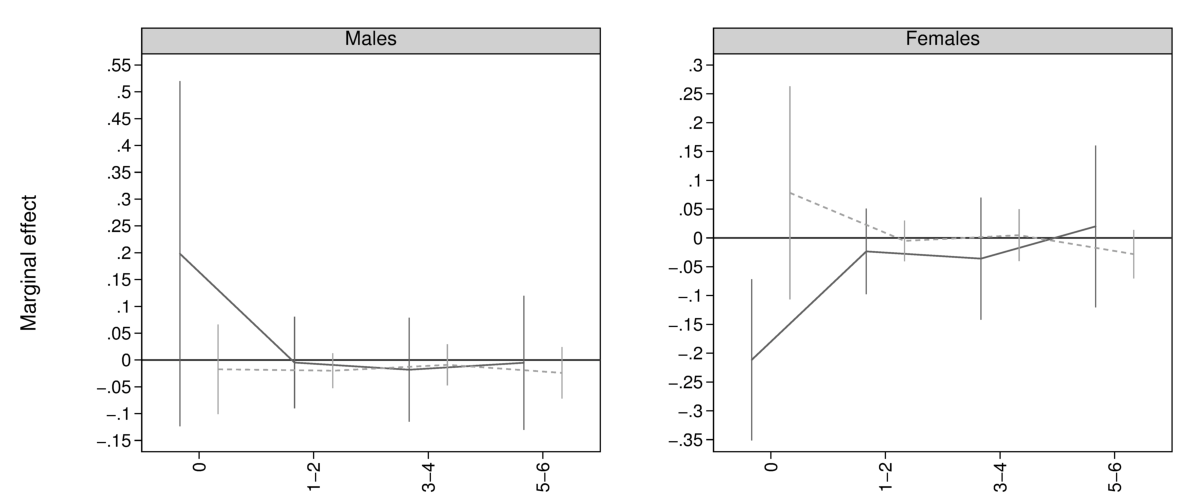
\includegraphics[width=\linewidth]{Chapter5/Figures/mi_msm_l_all_obese.pdf}
Fixed effects
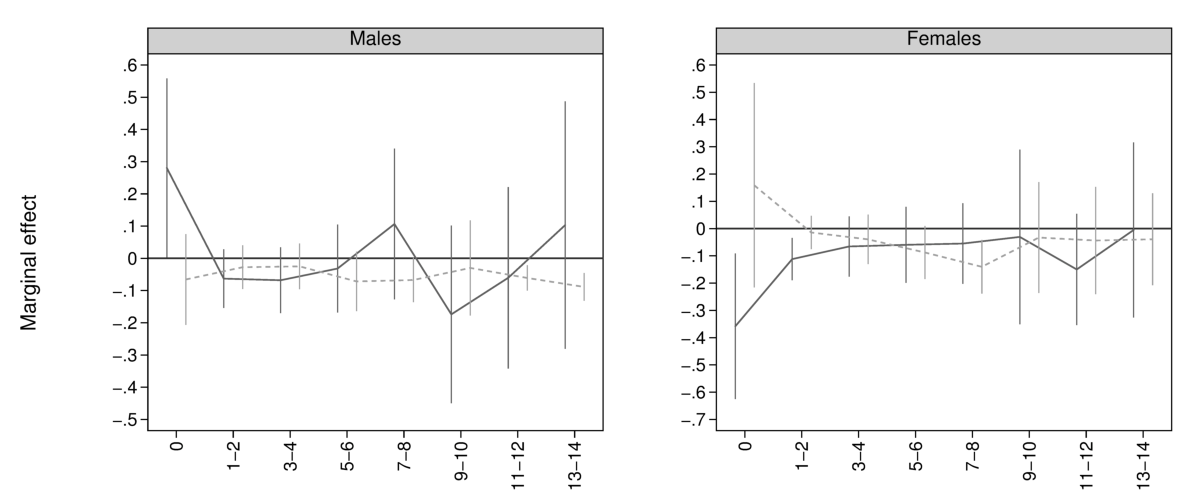
\includegraphics[width=\linewidth]{Chapter5/Figures/mi_obese_fe.pdf}
Random effects
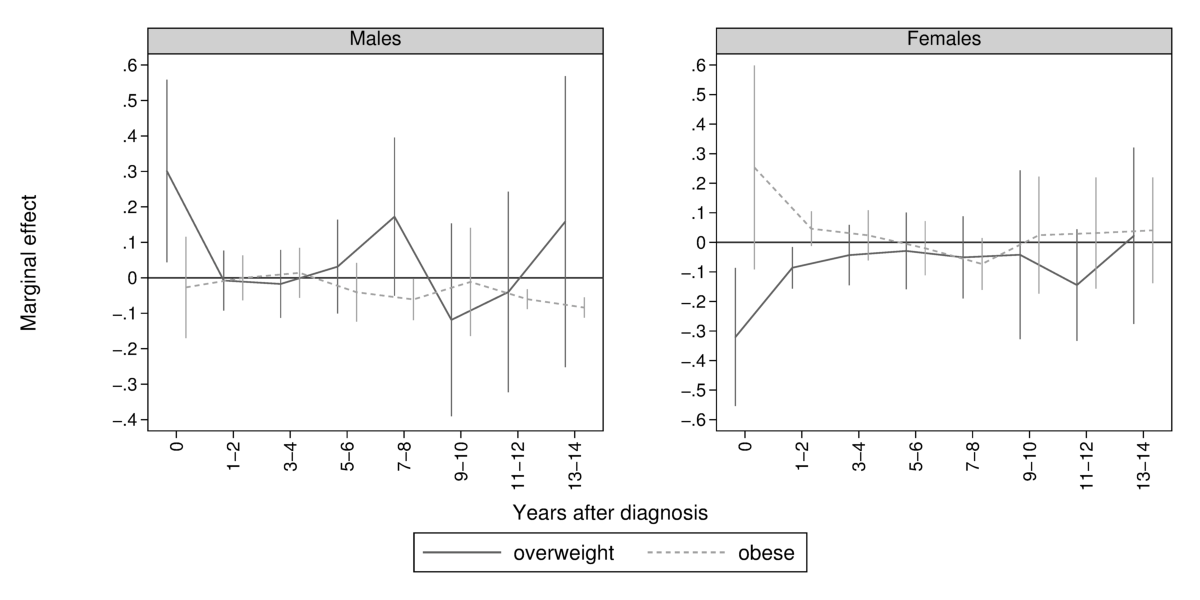
\includegraphics[width=\linewidth]{Chapter5/Figures/mi_obese_re.pdf}
\footnotesize{Notes: For MSM, effects after 6 years could not be estimated due to too few observations.}
\end{center}
\end{figure}
\clearpage